%!TEX root = ../report.tex
%%%%%%%%%%%%%%%%%%%%%%%%%%%%%%%%%%%%%%%%%%%%%%%%%%%%%%%%%%%%%%%%%%%%%%%
%%%%%%%%%%%%%%%%%%%%%%%%%%%%%%%%%%%%%%%%%%%%%%%%%%%%%%%%%%%%%%%%%%%%%%%
%%%%%                                                                 %
%%%%%     <file_name>.tex                                             %
%%%%%                                                                 %
%%%%% Author:      <author>                                           %
%%%%% Created:     <date>                                             %
%%%%% Description: <description>                                      %
%%%%%                                                                 %
%%%%%%%%%%%%%%%%%%%%%%%%%%%%%%%%%%%%%%%%%%%%%%%%%%%%%%%%%%%%%%%%%%%%%%%
%%%%%%%%%%%%%%%%%%%%%%%%%%%%%%%%%%%%%%%%%%%%%%%%%%%%%%%%%%%%%%%%%%%%%%%

\chapter{Task Description}
\begin{figure}[h!]
  \centering 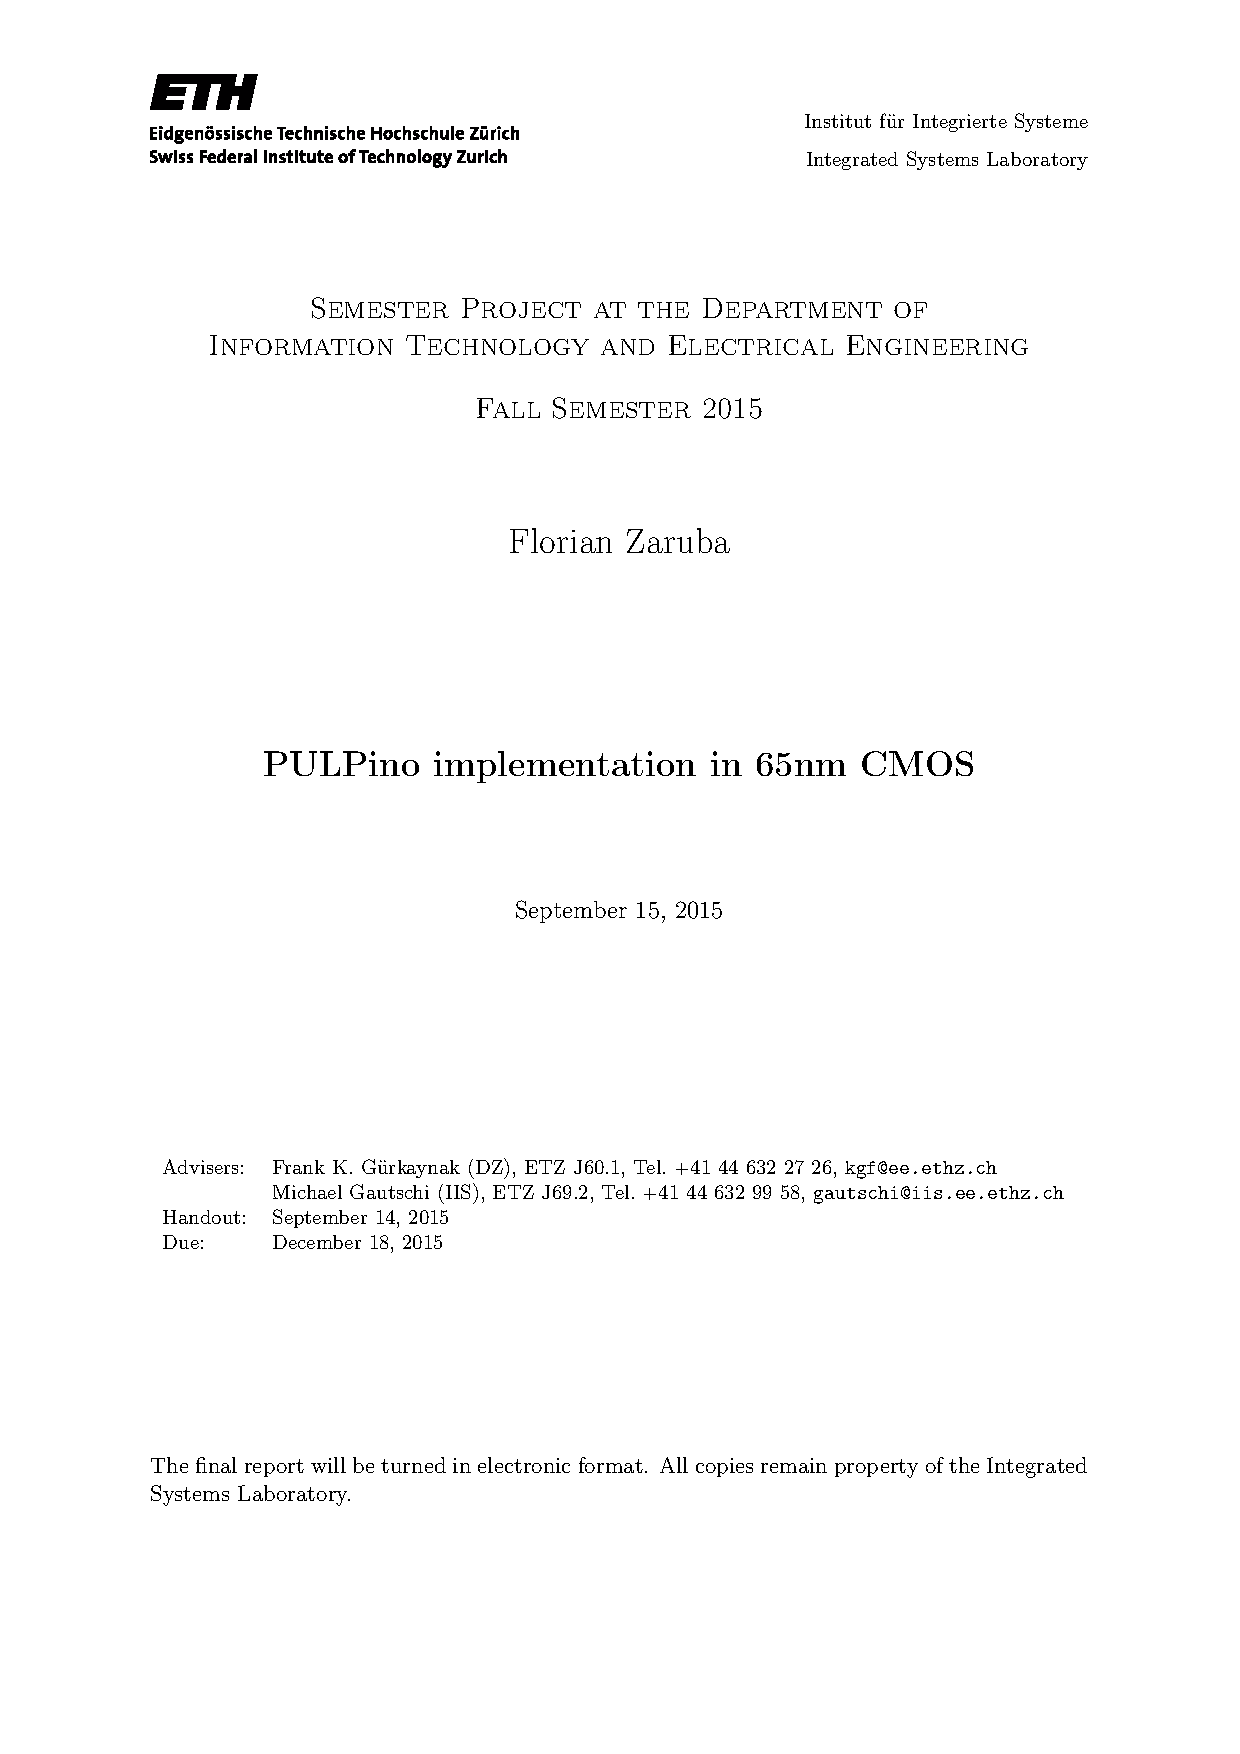
\includegraphics[width=0.55\textwidth]{task/TaskDescription.pdf}
 \end{figure}

\includepdf[pages={2-}, pagecommand={\thispagestyle{headings}}, turn=false, scale=0.9]{task/TaskDescription.pdf}

\chapter{Declaration of Originality}\label{chap:originality}
% include the signed declaration of authorship!


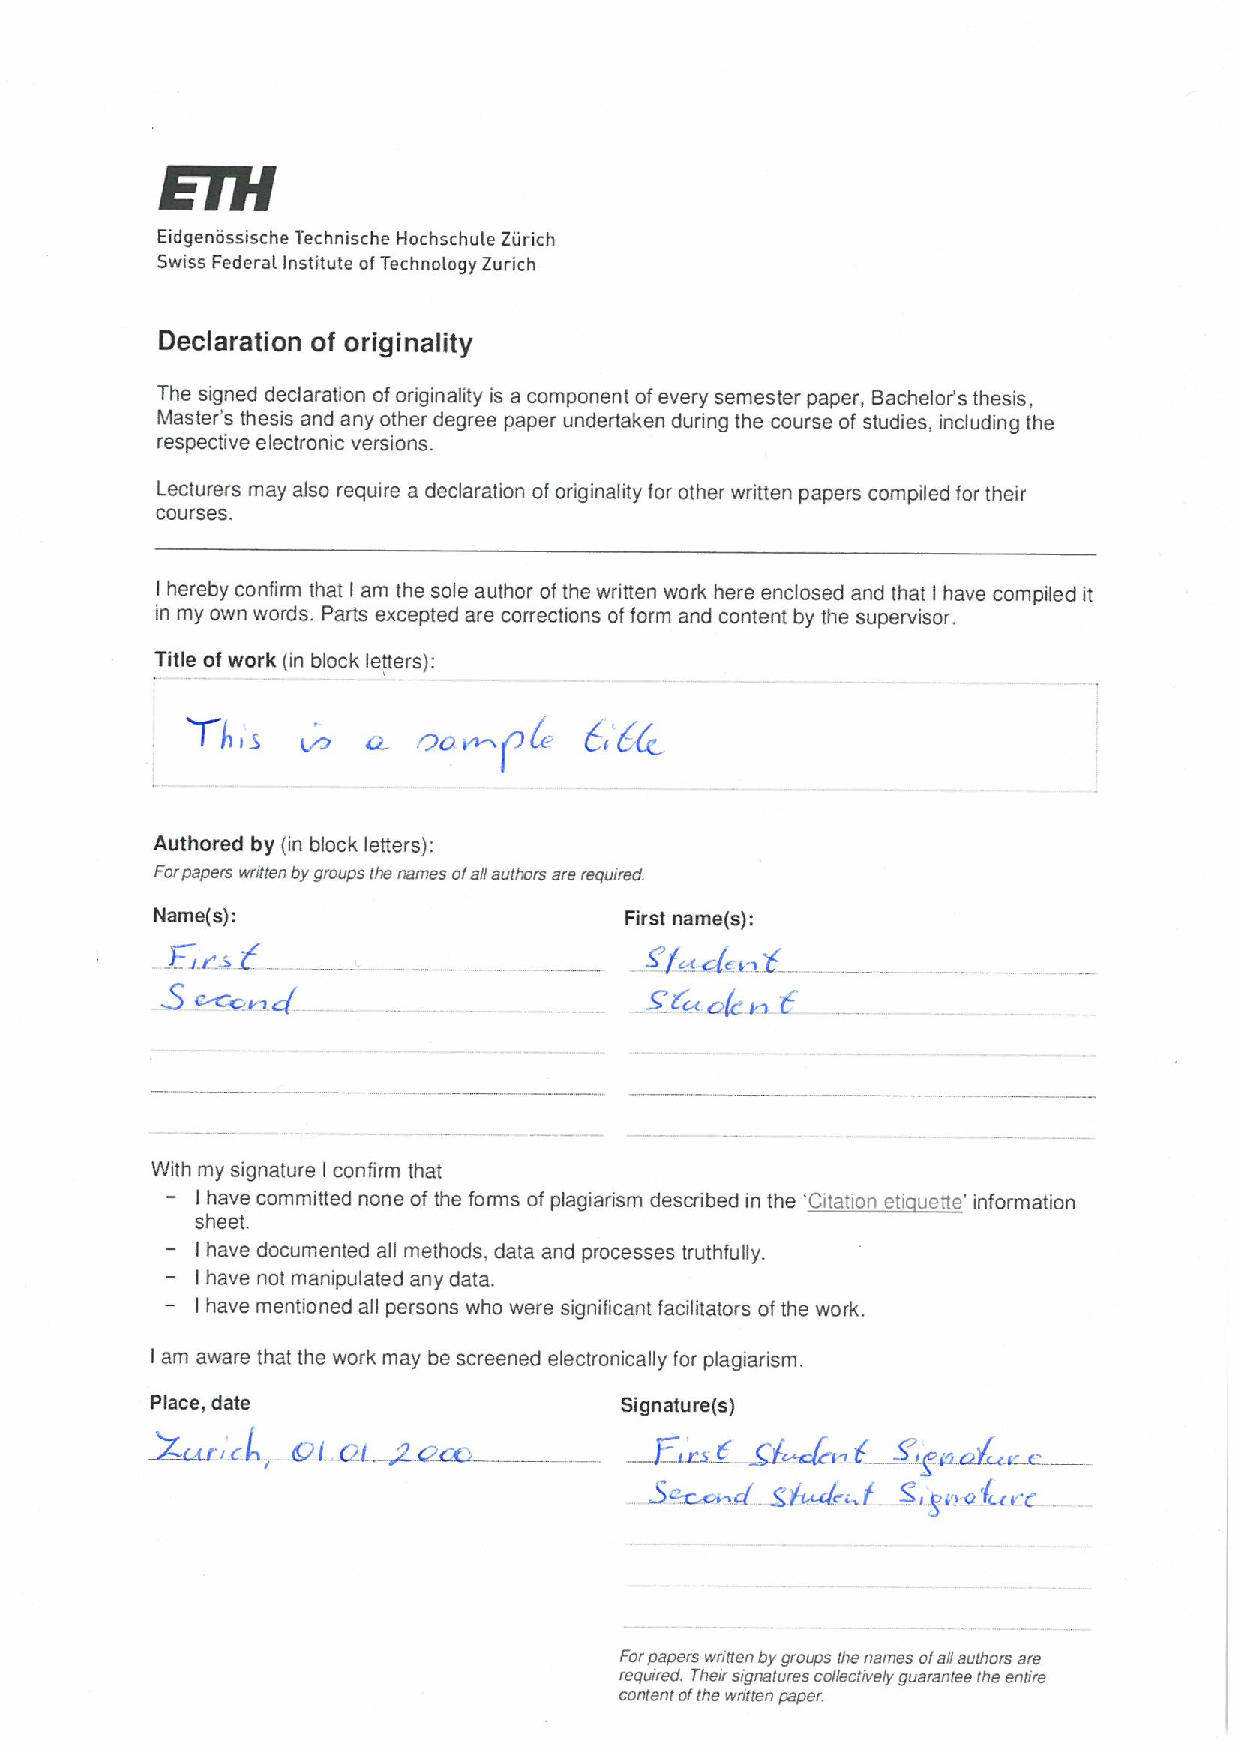
\includepdf[pages=-, turn=false, scale=0.9]{./figures/declaration_of_originality}
%\includepdf[pages={2-}, pagecommand={\thispagestyle{headings}}, turn=false, scale=0.9]{content/task.pdf} % 

% \section{File Structure}
% Describe how the project directories/files are organized, e.g.:

% \begin{flushleft}
% \dirtree{%
% .1 /.
%   .2 README \DTcomment{A README with some general information about the project.}.
%   .2 01\_report \DTcomment{The source files of the project report.}.
%   .2 02\_presentation \DTcomment{The source files of the presentation.}.
%   .2 03\_designflow \DTcomment{Some designflow-specific files.}.
% }
% \end{flushleft}

% What needs to be done to run an RTL simulation (stimuli generation,
% compilation...)?


\chapter{Datasets}
% If you have a data set comprising several test images, you could
% depict and describe them here. Use a simple naming scheme such that
% you can easily refer to certain elements of this data set in the text.


\section{More Evaluation Results}
% If you conducted an extensive evaluation you could move surplus
% graphs/results to the appendix.


\section{Algorithms / Tables}
% Large algorithm boxes and tables may clutter your chapters and impair
% the readability. If they are not very important, consider moving them
% to the appendix as well.

\section{Boot code}
\label{sec:boot_code}
\lstinputlisting[language=C, numbers=left, keywordstyle=\color{blue}]{../../sw/apps/boot_code/boot_code.c}
